\documentclass[man]{apa6}
\usepackage{lmodern}
\usepackage{amssymb,amsmath}
\usepackage{ifxetex,ifluatex}
\usepackage{fixltx2e} % provides \textsubscript
\ifnum 0\ifxetex 1\fi\ifluatex 1\fi=0 % if pdftex
  \usepackage[T1]{fontenc}
  \usepackage[utf8]{inputenc}
\else % if luatex or xelatex
  \ifxetex
    \usepackage{mathspec}
  \else
    \usepackage{fontspec}
  \fi
  \defaultfontfeatures{Ligatures=TeX,Scale=MatchLowercase}
\fi
% use upquote if available, for straight quotes in verbatim environments
\IfFileExists{upquote.sty}{\usepackage{upquote}}{}
% use microtype if available
\IfFileExists{microtype.sty}{%
\usepackage{microtype}
\UseMicrotypeSet[protrusion]{basicmath} % disable protrusion for tt fonts
}{}
\usepackage{hyperref}
\hypersetup{unicode=true,
            pdftitle={Infants' preference for speech decomposed: Meta-analytic evidence},
            pdfauthor={Cécile Issard, Sho Tsuji, \& Alejandrina Cristia},
            pdfkeywords={Meta-analysis, infants, speech preference, auditory development, natural
sounds},
            pdfborder={0 0 0},
            breaklinks=true}
\urlstyle{same}  % don't use monospace font for urls
\usepackage{graphicx,grffile}
\makeatletter
\def\maxwidth{\ifdim\Gin@nat@width>\linewidth\linewidth\else\Gin@nat@width\fi}
\def\maxheight{\ifdim\Gin@nat@height>\textheight\textheight\else\Gin@nat@height\fi}
\makeatother
% Scale images if necessary, so that they will not overflow the page
% margins by default, and it is still possible to overwrite the defaults
% using explicit options in \includegraphics[width, height, ...]{}
\setkeys{Gin}{width=\maxwidth,height=\maxheight,keepaspectratio}
\IfFileExists{parskip.sty}{%
\usepackage{parskip}
}{% else
\setlength{\parindent}{0pt}
\setlength{\parskip}{6pt plus 2pt minus 1pt}
}
\setlength{\emergencystretch}{3em}  % prevent overfull lines
\providecommand{\tightlist}{%
  \setlength{\itemsep}{0pt}\setlength{\parskip}{0pt}}
\setcounter{secnumdepth}{0}
% Redefines (sub)paragraphs to behave more like sections
\ifx\paragraph\undefined\else
\let\oldparagraph\paragraph
\renewcommand{\paragraph}[1]{\oldparagraph{#1}\mbox{}}
\fi
\ifx\subparagraph\undefined\else
\let\oldsubparagraph\subparagraph
\renewcommand{\subparagraph}[1]{\oldsubparagraph{#1}\mbox{}}
\fi

%%% Use protect on footnotes to avoid problems with footnotes in titles
\let\rmarkdownfootnote\footnote%
\def\footnote{\protect\rmarkdownfootnote}


  \title{Infants' preference for speech decomposed: Meta-analytic evidence}
    \author{Cécile Issard\textsuperscript{1}, Sho Tsuji\textsuperscript{2}, \&
Alejandrina Cristia\textsuperscript{1}}
    \date{}
  
\shorttitle{Preference for speech sounds in infancy}
\affiliation{
\vspace{0.5cm}
\textsuperscript{1} Laboratoire de Sciences Cognitives et Psycholinguistique, Ecole Normale Supérieure, Département d'Études Cognitives\\\textsuperscript{2} International Research Center for Neurointelligence, The University of Tokyo}
\keywords{Meta-analysis, infants, speech preference, auditory development, natural sounds\newline\indent Word count: 4400}
\usepackage{csquotes}
\usepackage{upgreek}
\captionsetup{font=singlespacing,justification=justified}

\usepackage{longtable}
\usepackage{lscape}
\usepackage{multirow}
\usepackage{tabularx}
\usepackage[flushleft]{threeparttable}
\usepackage{threeparttablex}

\newenvironment{lltable}{\begin{landscape}\begin{center}\begin{ThreePartTable}}{\end{ThreePartTable}\end{center}\end{landscape}}

\makeatletter
\newcommand\LastLTentrywidth{1em}
\newlength\longtablewidth
\setlength{\longtablewidth}{1in}
\newcommand{\getlongtablewidth}{\begingroup \ifcsname LT@\roman{LT@tables}\endcsname \global\longtablewidth=0pt \renewcommand{\LT@entry}[2]{\global\advance\longtablewidth by ##2\relax\gdef\LastLTentrywidth{##2}}\@nameuse{LT@\roman{LT@tables}} \fi \endgroup}


\DeclareDelayedFloatFlavor{ThreePartTable}{table}
\DeclareDelayedFloatFlavor{lltable}{table}
\DeclareDelayedFloatFlavor*{longtable}{table}
\makeatletter
\renewcommand{\efloat@iwrite}[1]{\immediate\expandafter\protected@write\csname efloat@post#1\endcsname{}}
\makeatother

\authornote{This work was supported by an Agence Nationale de
la Recherche grant to A.C. (ANR-17-CE28-0007 LangAge, ANR-16-DATA-0004
ACLEW, ANR-14-CE30-0003 MechELex, ANR-17-EURE-0017); and the J. S.
McDonnell Foundation Understanding Human Cognition Scholar Award to A.C.

The authors declare no conflict of interest. Funding sources did not
take part in study design, data collection or analysis.

Our data is fully available in the corresponding OSF repository:
\url{http://tidy.ws/bqjc4U}

Correspondence concerning this article should be addressed to Cécile
Issard, Laboratoire de Sciences Cognitives et Psycholinguistique,
Département d'Études Cognitives, Ecole Normale Supérieure, 29 rue d'Ulm,
75005 Paris, France. E-mail:
\href{mailto:cecile.issard@gmail.com}{\nolinkurl{cecile.issard@gmail.com}}}

\abstract{
The human auditory system is amazingly efficient at processing speech,
with a preference for these sounds reported by full term birth. Numerous
studies have investigated this preference at a variety of ages, and with
a large variety of sounds contrasted to speech, from monkey calls to
white noise. Many of these contrasts confound familiar, natural, and/or
vocal sounds, inviting a meta-analytic analyses in which these three
conceptually distinct explanations (preference for familiar, natural, or
vocal sounds) are statistically tested. Moreover, when analyzed in a
piecemeal fashion, previous experimental work suggested that infants'
preference for speech would initially encompass a broad range of natural
or vocal sounds, and then tune in to species-specific vocalizations,
namely speech. A meta-analytic framework allows us to check whether this
explanation holds for the entire body of literature. We therefore
synthesized the literature by conducting a meta-analysis of studies
testing speech preference in infants from birth to one year of age. We
found a medium effect size, with infants preferring speech over other
sounds. This preference was not significantly moderated by familiarity
with the language of the speech sound, vocal quality, or naturalness of
the competitor. We found no effect of age: infants showed the same
strength of preference throughout the first year of life. Speech
therefore appears to be preferred from birth, even to other natural or
vocal sounds. These results contradict current views of the literature,
and call for further investigation of the phenomenon, especially in
older infants.


}

\begin{document}
\maketitle

\section{Highlights}\label{highlights}

\begin{itemize}
\tightlist
\item
  Infants reliably prefer natural speech over other types of sounds,
  from birth to the end of the first year of life
\item
  Speech is preferred over both artificial and other natural sounds
\item
  Speech is preferred over both non-vocal and other vocal sounds
\item
  The difference between whether infants are familiar or not with the
  language used was not significant
\end{itemize}

\section{Introduction}\label{introduction}

Speech is a crucial signal for human vocal communication and social
interactions. Previous work argued for an early precursor of such social
interactions, manifested as a preference for speech over other types of
sound from birth (Ecklund-Flores \& Turkewitz, 1996; Vouloumanos \&
Werker, 2007; Vouloumanos, Hauser, Werker, \& Martin, 2010). This
auditory bias would initially encompass a broad range of natural or
vocal sounds (Figure 1), and then tune in to species-specific
communicative vocalizations, namely speech (e.g. Ferry, Hespos, \&
Waxman, 2013; Shultz \& Vouloumanos, 2010; Shultz, Vouloumanos, Bennett,
\& Pelphrey, 2014; Vouloumanos \& Werker, 2004; Vouloumanos et al.,
2010). However, statements about the factors driving this phenomenon are
often done using the demonstrably problematic method of concluding that
there is an interaction without actually testing for it statistically
(Gelman \& Stern, 2006). Here, we synthesize the available empirical
data on infants' preferences for speech over non-speech sounds to assess
the explanatory role of the factors cited in the literature.

\begin{figure}
\centering
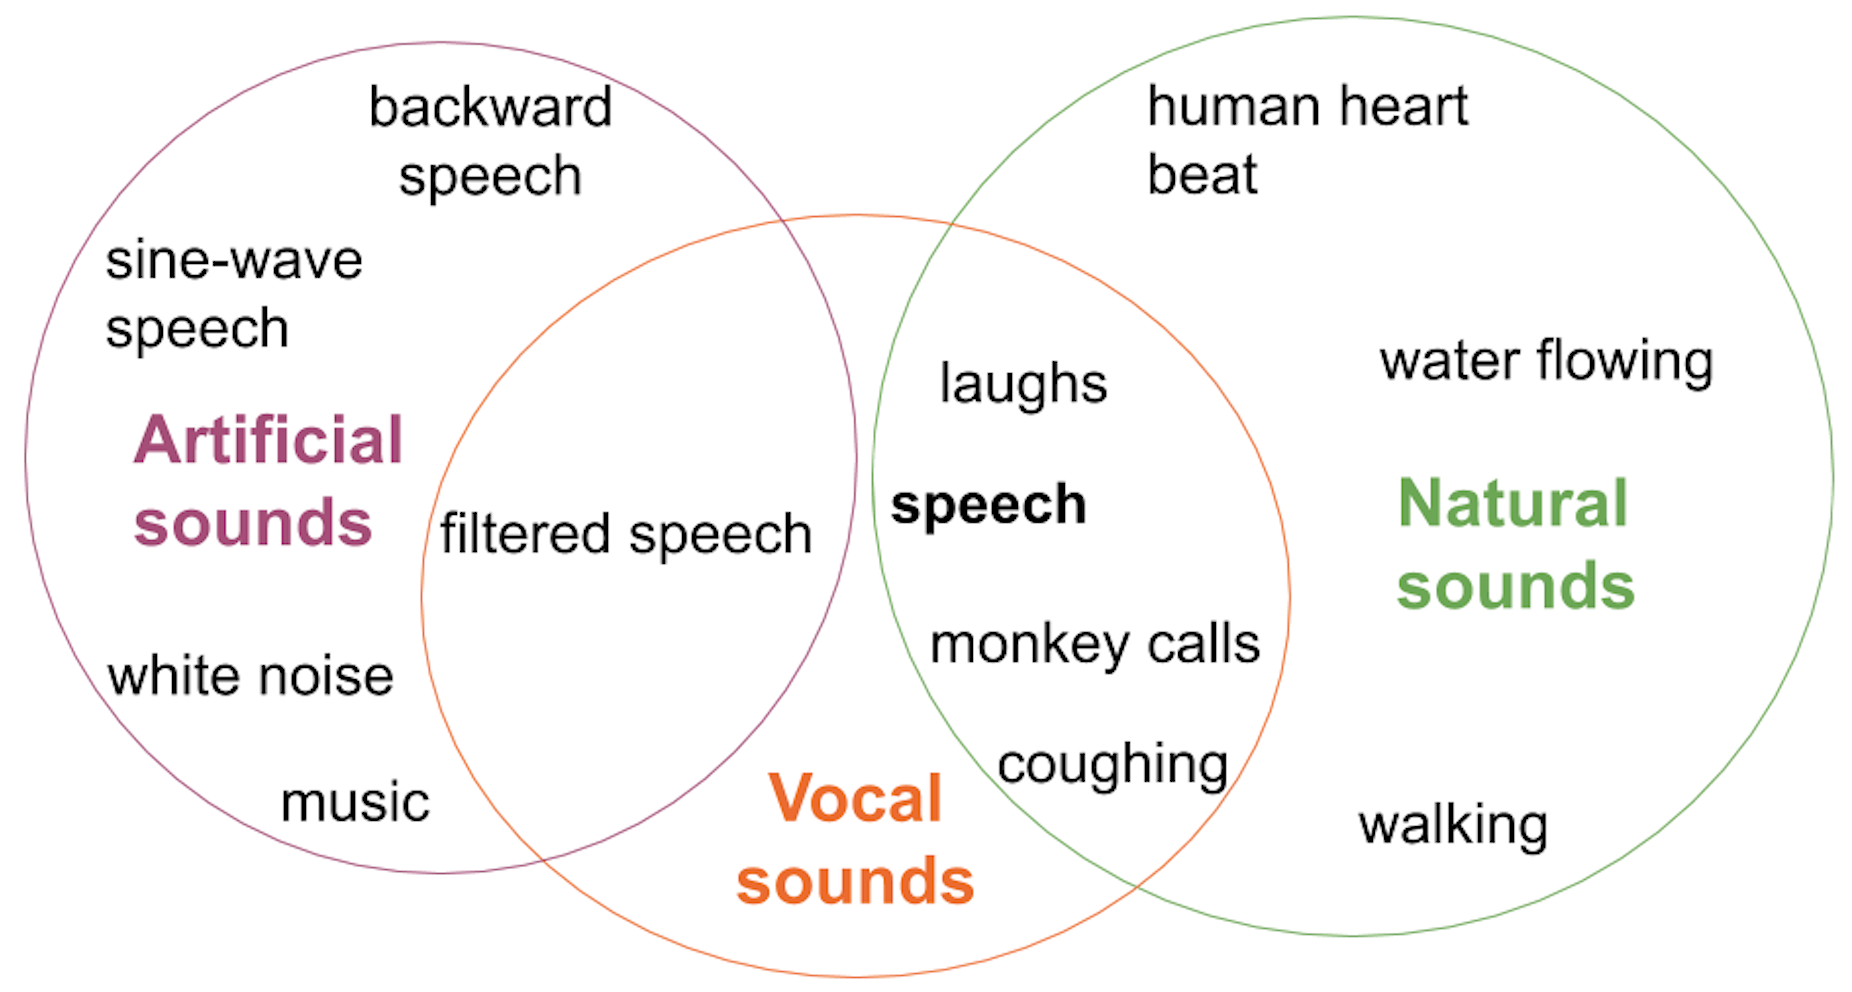
\includegraphics{/Users/Cecile/Documents/MA_speech_pref/figures_intro/Venn.png}
\caption{\label{fig:unnamed-chunk-1}Speech is a natural, vocal sound.}
\end{figure}

\subsection{Potential dimensions underlying preference
patterns}\label{potential-dimensions-underlying-preference-patterns}

\subsubsection{Familiarity}\label{familiarity}

A first hypothesis is that infants prefer speech to other sounds since
it is a frequent sound in their experience. Newborns prefer their native
speech to prosodically distinct foreign speech (e.g., Mehler et al.,
1988; Moon, Cooper, \& Fifer, 1993), which supports a preference for
sound patterns heard frequently in the womb. If this is the case,
infants would show a stronger preference for speech over other sounds
when tested in their native language, and a weaker preference when
tested with a foreign language. Two different studies testing
three-month-old infants with the same stimuli found a similar amount of
preference as compared to monkey calls whether speech was in the native
language (Vouloumanos et al., 2010) or a foreign language (Shultz \&
Vouloumanos, 2010), but results from neuroimaging studies provide
contradictory evidence. Newborns' brain activation was different for
forward than backward speech when the native language was used as the
speech stimuli, but not when a foreign language was used (May, Gervain,
Carreiras, \& Werker, 2018). It is therefore likely that this factor
drives infants' preference for speech, in interaction with properties of
the competitor.

\subsubsection{Naturalness}\label{naturalness}

A second hypothesis postulates a preference for natural over artificial
sounds. Natural sounds are those produced by biological systems, such as
environmental sounds, the sound of walking or heart beat. Natural sounds
are processed more efficiently by the auditory system, from the cochlea
(Smith \& Lewicki, 2006) to the auditory cortex (see Mizrahi, Shalev, \&
Nelken, 2014 for a review). As a result, this should be reflected in
infants behavior, with a preference for speech over artificial
competitors that is present from birth. Consistently, newborns increased
their sucking rate more during speech than during sine-wave speech
(Vouloumanos \& Werker, 2007), and three-month-olds did not listen
significantly longer to speech than to environmental sounds (Shultz \&
Vouloumanos, 2010). However, three-month-olds listened longer to speech
than to water sounds (Shultz \& Vouloumanos, 2010), and newborns made
more head-turns to speech than to heartbeat (Ecklund-Flores \&
Turkewitz, 1996). This suggests that from birth, infants have already
formed a narrower category within natural sounds.

\subsubsection{Vocal quality}\label{vocal-quality}

Perhaps the most widely cited hypothesis across the literature is that
of an initial preference for vocal sounds in general, that later
restricts to speech (e.g. Vouloumanos et al., 2010). Vocal sounds are
characterized by modulations introduced by the vocal tract, with
harmonically related energy peaks. In contrast, backward speech has
unnatural formant transitions and seemingly abrupt closures that cannot
be produced by the vocal tract\footnote{In the case of filtered speech,
  the modulations introduced by the vocal tract are still present at the
  retained frequencies, and formant transitions are consistent with
  vocal production constraints. For this reason, filtered speech can be
  considered as vocal but not natural. Because the womb acts as a
  low-pass filter, newborn infants are familiar with low-pass filtered
  speech, but this familiarity fades after birth.}. Accordingly,
newborns listened equivalently to speech and monkey calls (Vouloumanos
et al., 2010), and neuro-imaging results failed to report differential
response to speech, human non-communicative vocalizations, and rhesus
calls in 1- to 4-month-old infants (Shultz et al., 2014).

\subsection{Changes as a function of
development}\label{changes-as-a-function-of-development}

Development may affect the preference for speech in various ways.
Whereas newborns do not prefer speech over monkey calls,
three-month-olds do (Vouloumanos et al., 2010). This suggests that as
they age, infants might develop an increasingly narrow definition of the
stimulus they prefer. In this case naturalness, familiarity, and vocal
quality effects should change as a function of age: Very close stimuli
(e.g., speech versus another natural sound) initially leads to a weak
preference, but, as infants age, this preference may be as strong as
that found for very different stimuli (e.g., speech versus an artificial
sound). Many articles discuss potential changes in the pattern of
preference as a function of age (e.g. Ferry et al., 2013; Shultz \&
Vouloumanos, 2010; Shultz et al., 2014). To our knowledge, only two
papers from the same laboratory include multiple age groups tested with
the exact same stimulus categories and procedure (Vouloumanos \& Werker,
2004; Vouloumanos et al., 2010). It is therefore important to directly
test these statements with larger datasets, ideally across the whole
literature.

\subsection{A meta-analytic approach}\label{a-meta-analytic-approach}

In sum, previous work on infants' preferences is broadly compatible with
preference for natural over artificial, vocal over non-vocal, and
familiar over unfamiliar sounds, potentially interacting with infants'
age. In this paper, we seek to directly test these interpretations of
the literature by employing a meta-analytic approach.

Meta-analyses involve combining studies that may vary in their
methodology. One limitation is therefore that one cannot isolate
specific variables as well as in direct experimentation. Therefore,
meta-analyses may miss subtle effects. Nonetheless, they have several
useful features. They can reveal small effects not obvious in individual
studies by combining them to obtain larger samples. Additionally, by
integrating data across different laboratories, they provide evidence
for the generalizability of effects across labs. Finally, meta-analyses
offer tools to detect publication bias in the literature.

Specifically for the present case, a meta-analysis allows to
statistically test different explanations. We can test the effect of
factors that are not part of the original design, by redescribing the
stimuli used as a function of those factors. For instance, a study
measuring preference for native speech over native backward speech
provides data on a natural versus artificial, as well as a vocal versus
non-vocal contrast. We can also draw a developmental timeline across the
age range covered by the literature.

Meta-analyses can even provide theoretical and empirical insights that
contradict qualitative reviews. For example, it has been proposed that
infants' preference for novel or familiar items related to infants' age
such that, all things equal, younger infants showed familiarity
preferences whereas older infants exhibited novelty preferences (Hunter
\& Ames, 1988). However, Bergmann and Cristia (2016) found stable
familiarity preferences for word segmentation in natural speech across
the first two years; and Black and Bergmann (2017) found a stable
novelty effect for artificial grammars implemented in synthesized
speech, whereas those implemented in natural speech led to stable
familiarity preferences. Meta-analyses are therefore important to
statistically and systematically test the theoretical predictions
proposed in qualitative reviews.

\subsection{The present study}\label{the-present-study}

Given the scarcity of direct evidence on the potential explanations laid
out above (naturalness, vocal quality, and familiarity, as a function of
age), we conducted a meta-analysis to test whether infants' preference
for speech sounds over other types of sounds is reliable in newborns,
and how it develops over the first year of life. Assuming all three
factors are true, and further assuming that the definition of the
preferred stimulus narrows with age, we predicted that infants will show
(see Figure 2):

\begin{enumerate}
\def\labelenumi{\arabic{enumi}.}
\tightlist
\item
  a greater preference for speech over natural sounds as a function of
  age, but a stable preference for speech over artificial sounds that is
  stable over development;
\item
  a greater preference for speech over other vocal sounds as a function
  of age, but a stable preference for speech over non-vocal sounds over
  development;
\item
  a greater preference for native speech over non-speech as a function
  of age, but a smaller preference for foreign speech over non-speech
  with age.
\end{enumerate}

\begin{figure}
\centering
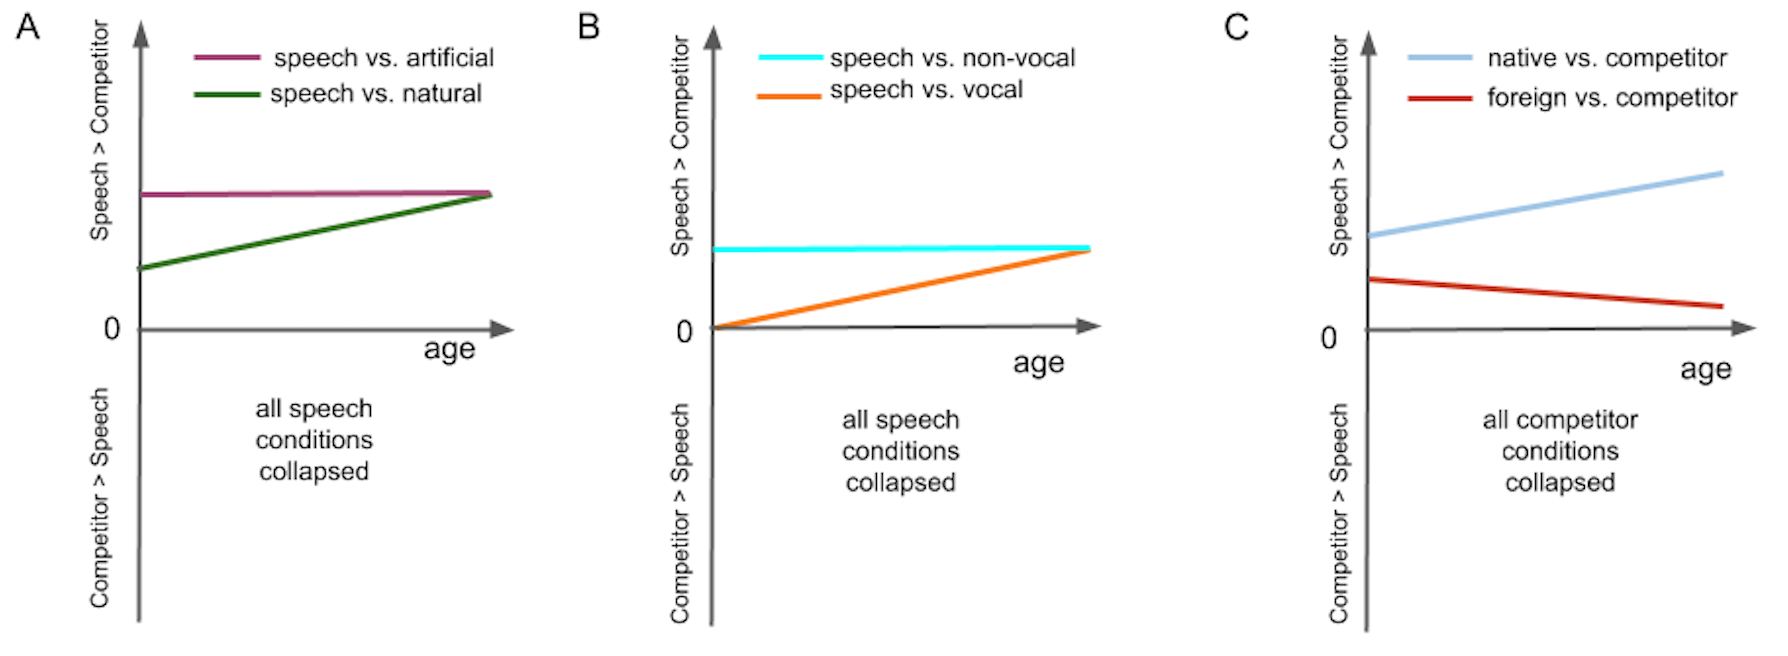
\includegraphics{/Users/Cecile/Documents/MA_speech_pref/figures_intro/hypotheses.png}
\caption{\label{fig:unnamed-chunk-2}Hypothesized pattern of preference: the
x axis shows age, the y axis represents the effect size derived from the
contrast between a speech condition and a competitor condition
(preference for speech over the competitor is plotted up; the lower
quadrants are empty because we do not predict a preference for the
competitor over speech). A: Speech contrasted to natural (green) or
artificial (purple) competitors. B: Speech contrasted to vocal (orange)
or non-vocal (cyan) competitors. C: Collapsing across competitors,
separating speech in a foreign language (red); speech in the native
language (blue).}
\end{figure}

\section{Methods}\label{methods}

\subsection{Literature search}\label{literature-search}

We composed the initial list of studies with suggestions by experts
(authors of this work); one google scholar search
(\emph{(\enquote{speech preference} OR \enquote{own-species
vocalization}) AND infant - \enquote{infant-directed}}), the same search
in PubMed and PsycInfo (last searched on 2019-09-24); and a google
alert. We also inspected the reference lists of all included papers.
Finally, we emailed a major mailing list to ask for missing data. We
received only two replies, one of which revealed a formerly undiscovered
published study, but no unpublished data was made available to us.

\subsection{Inclusion criteria}\label{inclusion-criteria}

After a first screening based on titles and abstracts using more liberal
inclusion criteria, we decided on inclusion based on full paper reading.
We included experiments that tested human infants from birth to one year
of age, and contrasted speech sounds with any other type of sound,
measuring behavioral preferences to the sounds (e.g., looking times). We
excluded experiments that did not contrast speech to another sound type,
such as studies contrasting two different speech sounds (e.g.~foreign
against native language, or adult vs.~child-directed speech), or on the
opposite did not present natural speech sounds at all (e.g.~backward
speech vs animal vocalizations). We excluded experiments that presented
speech in the mother's voice to avoid counfounds with voice recognition.
Experiments that intentionally mixed speech with other vocal sounds
within the same sound condition were also excluded. Finally, we excluded
neuroimaging studies to avoid mixing results from different brain
regions with different response profiles. We included published (i.e.,
journal articles) as well as unpublished works (i.e., doctoral
dissertations as long as sufficient information was provided).

A PRISMA flow chart summarizes the literature review and selection
process (Figure 3). We documented all the studies that we inspected in a
decision spreadsheet (available in the online supplementary materials;
\url{https://osf.io/4stz9/?view_only=d0696591ebf34bfc8430f848cd945ca8}).

\begin{figure}
\centering
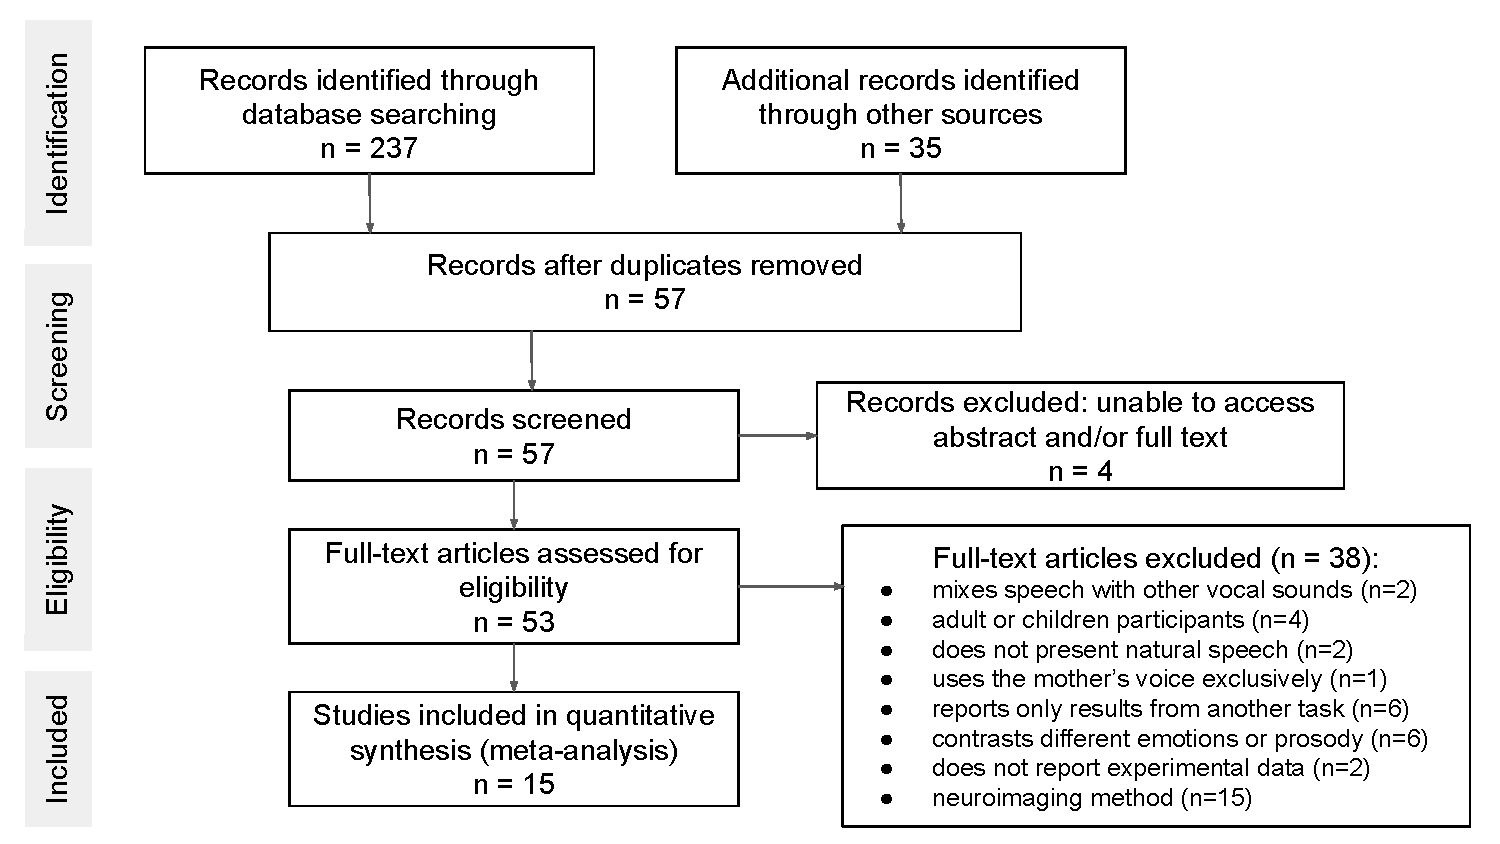
\includegraphics{/Users/Cecile/Documents/MA_speech_pref/figures_intro/PRISMA.pdf}
\caption{\label{fig:unnamed-chunk-3}PRISMA flowchart summarizing the
literature review and selection process.}
\end{figure}

\subsection{Coding}\label{coding}

The critical variables for our purpose are infant age, methodological
variables (testing method: central fixation, high amplitude sucking,
head-turn preference procedure, high amplitude sucking/passive
listening), and key stimuli characteristics. Specifically, we coded the
language in which the speech sounds were recorded (native or foreign),
and whether the sound opposed to speech was natural or not, vocal or
not. This competitor was coded as natural if it was produced by a
biological organism without any further acoustic manipulation. If the
authors applied acoustic manipulations it was coded as artificial. This
sound was considered as vocal if it was produced by an animal vocal
tract, either original or modified. If a paper reported results from
neurotypical and at-risk infants, we coded only the data from the
neurotypical group.

Data were coded by the first author. In addition, 20\% of the papers
were randomly selected to be coded by the last author independently,
with disagreements resolved by discussion. There were 10 disagreements
out of a total of 260 fields filled in, and they were indicative of the
coders not following the codebook, which led to a revision of all data
in four variables.

We coded all the statistical information reported in the included
papers. If reported, we coded the mean score and the standard deviation
for speech, and the other sound separately. When infant-level data was
provided, we recomputed the respective mean scores and standard
deviations based on the reported individual scores. If reported, we also
coded the t-statistic between the two sound conditions, or an
F-statistic provided this was a two-way comparison. If effect sizes were
directly reported as a Cohen's d or a Hedges' g, we also coded this.

The PRISMA checklist, data, and code can be found on the online
supplementary materials
(\url{https://osf.io/4stz9/?view_only=d0696591ebf34bfc8430f848cd945ca8}).

\subsection{Effect sizes}\label{effect-sizes}

Once the data were coded, we extracted effect sizes, along with their
respective variance. Effect sizes were standardized differences (Cohen's
d) between response to speech and to the other sound. If they were not
directly reported in the papers, we computed them using the respective
means and SDs (Lipsey \& Wilson, 2001), or a t- or F-statistic (Dunlap,
Cortina, Vaslow, \& Burke, 1996). As our effect sizes came from
within-subject comparisons (e.g.~looking time of the same infant during
speech and during monkey calls), we needed to take into account the
correlation between the two measurements in effect sizes and effect size
variances computations. We computed this correlation based on the
t-statistic, the respective means and SDs (Lipsey \& Wilson, 2001) if
they were all reported; or imputed this correlation randomly if not. We
finally calculated the variance of each effect size (Lipsey \& Wilson,
2001). Cohen's d were transformed to Hedges' g by multiplying d by a
correction for small sample sizes based on the degree of freedom
(Borenstein, Hedges, Higgins, \& Rothstein, 2011).

All analyses use the R (R Core Team, 2018) package Robumeta (Hedges,
Tipton, \& Johnson, 2010), which allows to fit meta-analytic regressions
that take into account the correlated structure of the data, when
repeated measures are obtained from the same infant groups within
papers.

\section{Results}\label{results}

\subsection{Database description}\label{database-description}

We found a total of 16 papers reporting 52 (not mutually independent)
effect sizes, see Figure 4. 15 papers have been submitted to or
published in peer-reviewed journals (Colombo \& Bundy, 1981; Cooper \&
Aslin, 1994; Curtin \& Vouloumanos, 2013; Ecklund-Flores \& Turkewitz,
1996; Santolin, Russo, Calignano, Saffran, \& Valenza, 2019; Segal \&
Kishon-Rabin, 2011; Shultz \& Vouloumanos, 2010; Sorcinelli, Ference,
Curtin, \& Vouloumanos, 2019; Spence \& DeCasper, 1987; Vouloumanos \&
Curtin, 2014; Vouloumanos \& Werker, 2004, 2007; Vouloumanos, Druhen,
Hauser, \& Huizink, 2009; Vouloumanos et al., 2010, 2010; Yamashiro,
Curtin, \& Vouloumanos, 2019). The remaining 1 paper contributing 1
effect size was a thesis (J. D. Ference, 2018).

Studies tended to have small sample sizes, with a median N of 15
children (Range = 56, M = 18.77, Total: 665). Infants ranged from 0 to
12 months (1.50 to 380.50 days), although the majority were under 9
months of age (75\% of the studies). Individual samples comprised 47\%
of female participants on average. Infants were native of 6 different
languages across the whole database (English, French, Russian, Yiddish,
Hebrew, Italian). Studies were performed in 10 different laboratories
from 4 different countries (United States, Canada, Israel, Italy). 3
experimental methods were used: 13 experiments used Central Fixation
(CF) (Colombo \& Bundy, 1981; Cooper \& Aslin, 1994; Curtin \&
Vouloumanos, 2013; J. D. Ference, 2018; Santolin et al., 2019; Segal \&
Kishon-Rabin, 2011; Shultz \& Vouloumanos, 2010; Sorcinelli et al.,
2019; Vouloumanos \& Curtin, 2014; Vouloumanos \& Werker, 2004;
Vouloumanos et al., 2009, 2010; Yamashiro et al., 2019); 3 used
High-Amplitude Sucking (HAS) (Spence \& DeCasper, 1987; Vouloumanos \&
Werker, 2007; Vouloumanos et al., 2010); and 1 used Head-turn Preference
Procedure (HPP) (Ecklund-Flores \& Turkewitz, 1996).

\subsection{Average effect size}\label{average-effect-size}

\begin{figure}
\centering
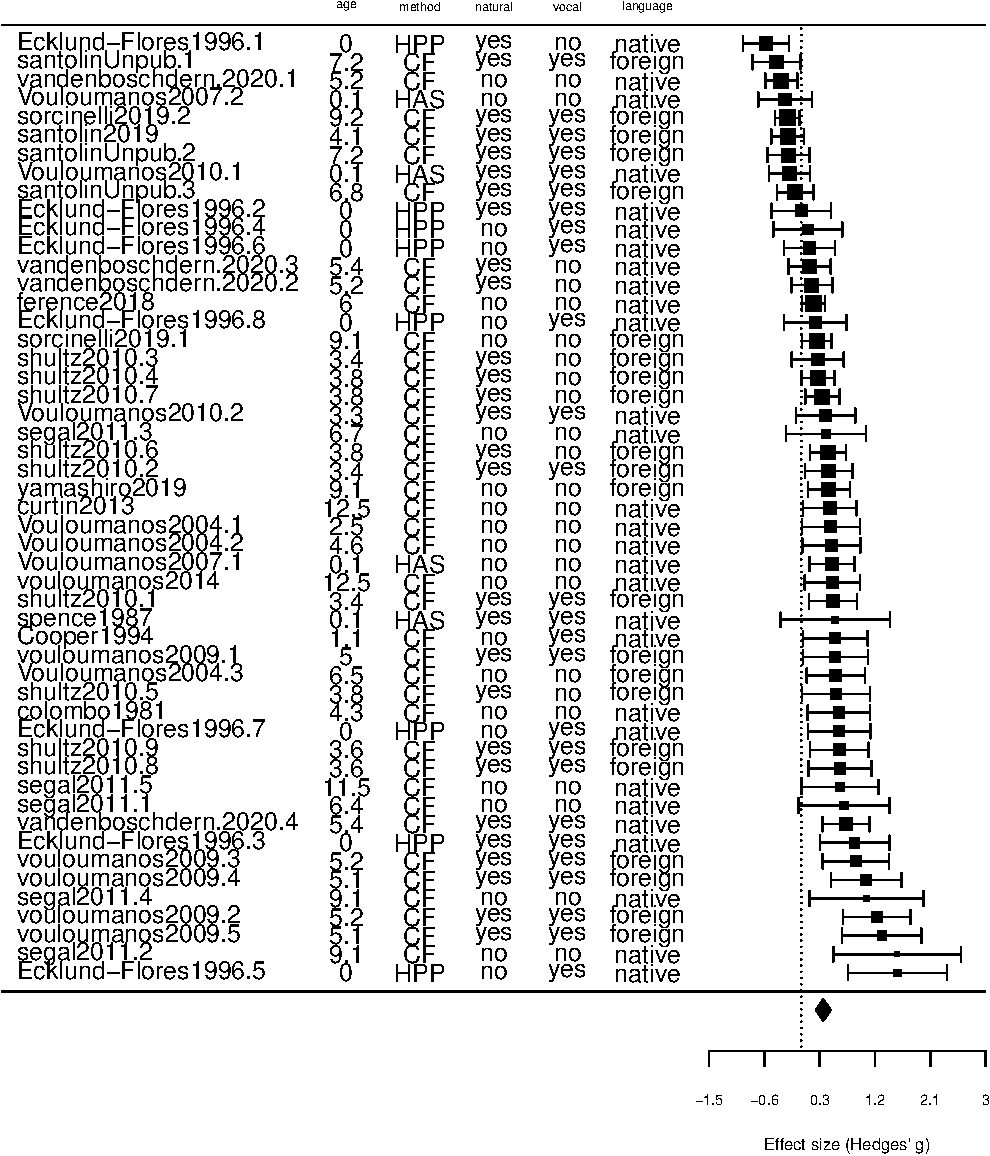
\includegraphics{MA_speech_pref_files/figure-latex/forest-1.pdf}
\caption{\label{fig:forest}Forest plot of effect sizes available in the
literature.}
\end{figure}

Integrating across all studies in a meta-analytic regression without any
moderator, we found an average effect size g of 0.42 (SE = 0.08, CI =
{[}0.26 , 0.57{]}) (Table 1, and Figure 4, diamond), corresponding to a
medium effect size.

\subsection{Publication bias}\label{publication-bias}

\begin{figure}
\centering
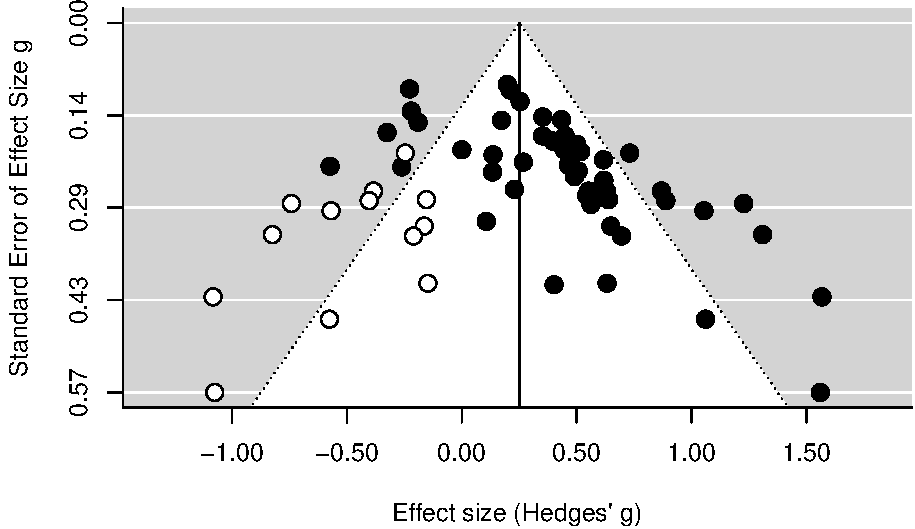
\includegraphics{MA_speech_pref_files/figure-latex/publication bias-1.pdf}
\caption{(\#fig:publication bias)Funnel plot for publication bias.}
\end{figure}

We assessed the presence of a potential publication bias in the body of
literature by studying the relationship between standard errors of
effect sizes as a function of Hedges' g (see funnel plot in Figure
5).\footnote{If the literature is not biased, effect sizes should be
  evenly distributed around the mean effect size, with increasing
  standard error as they go away from the mean effect size (both in the
  positive and negative directions, white triangle in the funnel plot).
  This is reflected by a symmetrical funnel plot, with no linear
  relationship between effect sizes and standard errors.} A regression
test on these data was significant (z = 7.27, p = 0.00), as was the
Kendall's tau rank correlation test for funnel plot asymmetry (Kendall's
tau = 0.53, p = 0.00), consistent with a publication bias in the
literature. To further investigate this bias, we symmetrized the funnel
plot with the \enquote{trim and fill} method (Duval \& Tweedie, 2000).
To symmetrize the funnel plot, 12 (SE = 4.33) missing studies were
needed on the left side of the plot.

\subsection{Moderator analyses}\label{moderator-analyses}

We then tested if the preference found above could be explained by the
dimensions discussed in the literature. Following our hypotheses, we fit
a meta-analytic model with the following moderators:

\begin{itemize}
\tightlist
\item
  mean age of children;
\item
  familiarity with the language used (native or foreign);
\item
  naturalness of the contrastive sound (coded as yes if it was natural
  and no otherwise);
\item
  vocal quality of the contrastive sound (coded as yes if it was vocal
  and no otherwise).
\end{itemize}

None of the moderators was significant (see Figures 6, 7, and 8; and
Table 1).

\begin{table}[tbp]
\begin{center}
\begin{threeparttable}
\caption{\label{tab:Table1}Statistical results of meta-regression with all main effects. The estimates correspond to changes in the intercept when the target stimuli are in the native language (familiarity); the competitor is artificial (naturalness); and the competitor is non-vocal (vocal quality).}
\begin{tabular}{lccclccclccclccclccc}
\toprule
 & estimate & SE & t & confidence interval\\
\midrule
average effect size & 0.42 & 0.08 & 5.48 & 0.26 - 0.57\\
familiarity & 0.11 & 0.17 & 0.65 & -0.27 - 0.49\\
naturalness & 0.17 & 0.20 & 0.83 & -0.29 - 0.62\\
vocal quality & -0.08 & 0.23 & -0.35 & -0.61 - 0.46\\
age & 0.00 & 0.00 & 0.15 & 0 - 0\\
\bottomrule
\end{tabular}
\end{threeparttable}
\end{center}
\end{table}

Due to the relatively low number of effect sizes available in the
literature, we did not add interactions with age to the model to avoid
overfitting. The confidence intervals of all conditions overlap almost
exactly across the tested ages, excluding the possibility of such
interactions (Figure 4, 5, and 6). The absence of interaction between
age and other moderators was confirmed by three separate models for each
moderator, that did not yield any significant effect or interaction
(Supplementary Results S1).

\begin{figure}
\centering
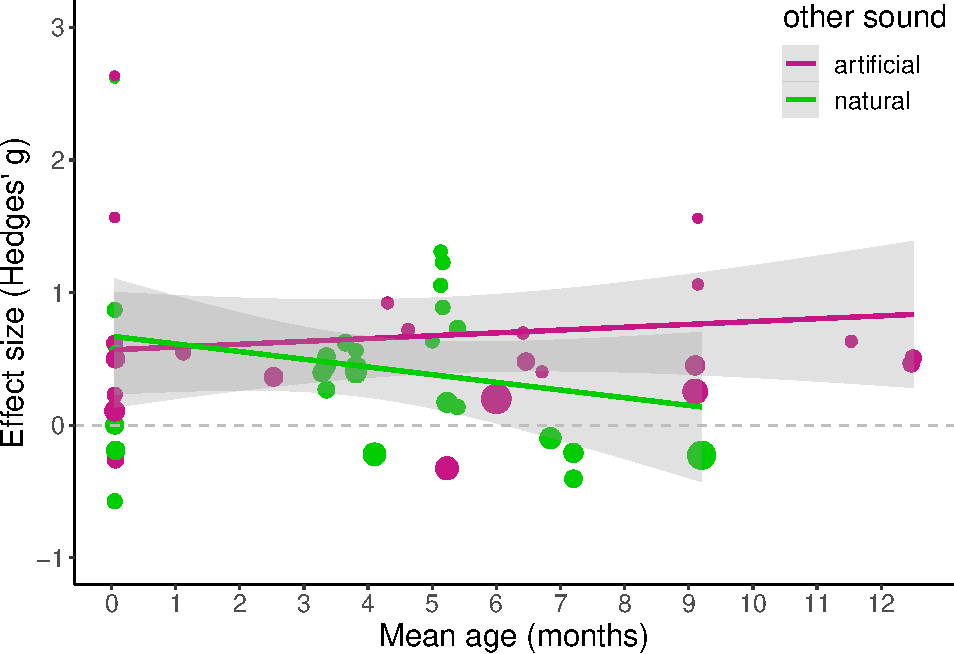
\includegraphics{MA_speech_pref_files/figure-latex/natural-1.pdf}
\caption{\label{fig:natural}Effect sizes as a function of age and natural
quality of the competitor}
\end{figure}

\begin{figure}
\centering
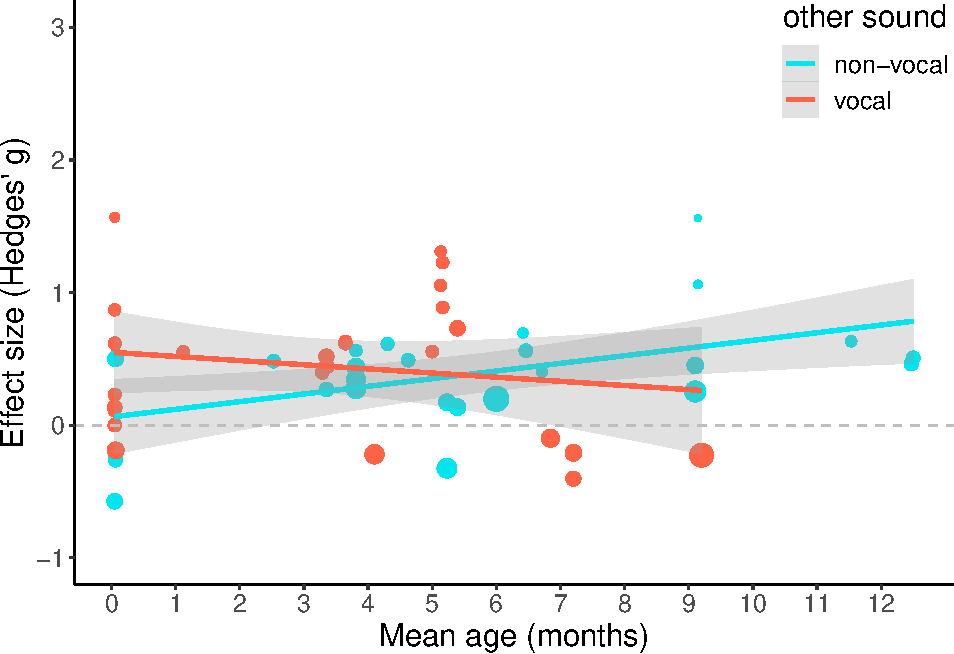
\includegraphics{MA_speech_pref_files/figure-latex/vocal-1.pdf}
\caption{\label{fig:vocal}Effect sizes as a function of age and vocal
quality of the competitor}
\end{figure}

\begin{figure}
\centering
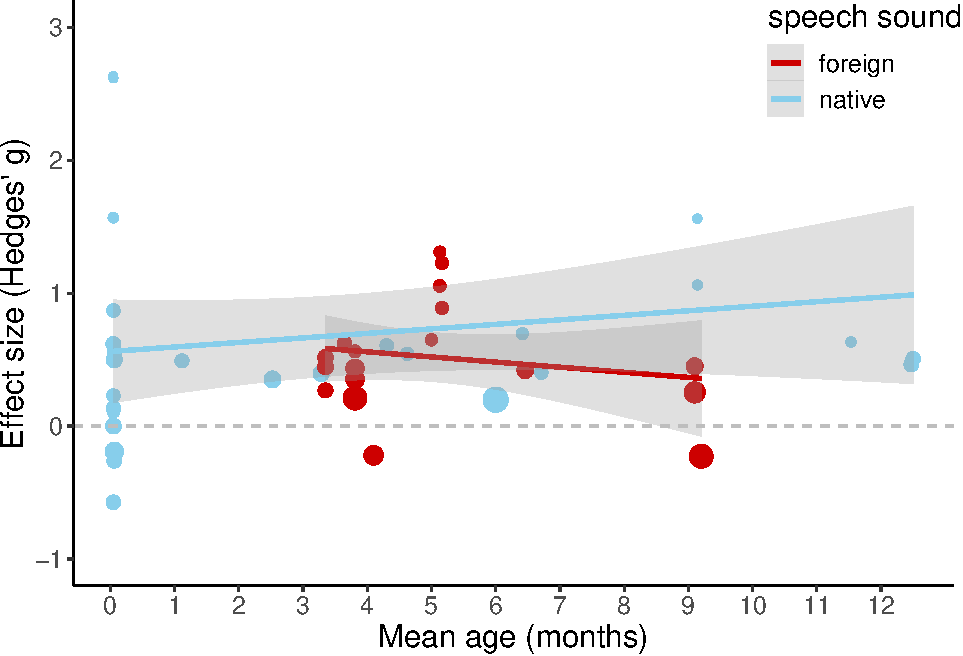
\includegraphics{MA_speech_pref_files/figure-latex/unnamed-chunk-4-1.pdf}
\caption{\label{fig:unnamed-chunk-4}Effect sizes as a function of age and
familiarity with the speech sounds.}
\end{figure}

Experimental method is known to be sizable in the cognitive
developmental literature (Bergmann et al., 2018). We assessed that it
did not impact our results by residualizing effect sizes from
experimental method (Supplementary figure S2).

\section{Discussion}\label{discussion}

Our meta-analysis synthesizes the available literature on infants'
preference for speech sounds. When all studies were considered together
with no moderators, we found a sizable intercept (g=0.42). For
comparison, the average effect for native vowel discrimination using
looking time methods is estimated at 0.25 (Tsuji \& Cristia, 2014, data
inspected in \url{http://metalab.stanford.edu} on 2019-10-18). We had
predicted infants' speech preference to be larger when the competitor
was an artificial sound than when it was a natural one; when the
competitor was non-vocal; and when the speech was in the infants' native
language. In fact, we were unable to disprove the null hypothesis of no
difference for all three factors. Distributions of effect sizes for
studies varying along the three dimensions widely overlap, and the
confidence intervals of all conditions overlap almost exactly (Figures
6, 7, and 8). Moreover, Table 1 shows that the estimate for all these
factors is close to zero (the maximum being 0.17). Our findings
therefore suggest that none of these parameters fully explain infants'
preference for speech sounds. These results are in line with adult
neuroimaging data showing distinct responses to speech as compared to
other natural or environmental sounds, even in low-level auditory
regions (Norman-Haignere \& McDermott, 2018; Norman-Haignere, Kanwisher,
\& McDermott, 2015).

We had also hypothesized age to play a major role, because it may
correlate with a reshaping of the category definition for speech itself.
Indeed, studies comparing processing of human speech against human
non-speech as well as animal vocalizations more generally (McDonald et
al., 2019; Vouloumanos et al., 2010) often discuss these age-related
differences in categorization of these sounds. Surprisingly, age did not
significantly moderate the overall preference for speech, as shown by
the null estimate of this moderator (Table 1). This result was
replicated in a separate model for age only, which showed an estimate
for the intercept similar to the intercept found in the meta-regression
with no moderator (Supplementary results S4). Moreover, the scatterplot
of effect sizes as a function of age reveals clearly no change with age
even when plotted without other moderators (Supplementary figure S5).
This null effect of age, combined with the sizeable intercept, confirms
that infants reliably prefer speech over other types of sounds from
birth.

In other words, from birth on, infants show a preference for speech,
which cannot be reduced to three simpler explanations: naturalness,
vocalness, or familiarity (represented here by comparing effects for
native versus competitor against those for foreign versus competitor).
This capacity to preferentially listen to speech sounds from birth
suggests that infants are born with the capacity to recognize their
conspecifics' communication signals. This parallels what has been
proposed by the Conspec model for faces: Infants would be born with
knowledge about faces, enabling them to orient their attention toward
them, even without any prior exposure to faces (Morton \& Johnson,
1991). A capacity to recognize conspecifics, either from their face or
their voice, is consistent with the similar processing stages between
voice and face perception (Yovel \& Belin, 2013). The fact that
familiarity with the language used in the experiment did not modulate
infants' preference suggests that exposure did not play a crucial role
for speech either. However, contrary to faces, fetuses are exposed to
speech that is low-pass filtered by the womb throughout the last
trimester of gestation (Lecanuet \& Granier-Deferre, 1993; Querleu,
Renard, Versyp, Paris-Delrue, \& Crèpin, 1988). It is therefore possible
that prenatal experience with low-pass filtered speech helps infants to
form a representation of speech, independently of the language spoken.

The Conspec model proposes that faces would be detected because of their
spatial structure (Morton \& Johnson, 1991). Similarly, it is possible
that infants prefer speech because of its complex acoustic structure and
fast transitions (Rosen \& Iverson, 2007). Spectral or temporal
modulations taken separately are not sufficient to elicit neural
responses similar to the ones elicited by speech (Minagawa-Kawai,
Cristià, Vendelin, Cabrol, \& Dupoux, 2011). However, speech is
characterized by joint spectrotemporal modulations at specific rates
(Singh \& Theunissen, 2003). It is possible that infants attune to this
specific spectro-temporal structure (though see Norman-Haignere \&
McDermott, 2018 showing that they only explain neural responses in
primary auditory cortex). Testing this explanation would require to
compute the modulation spectra of the actual stimuli used in the
studies. Thus, we recommend interested researchers to deposit their
stimuli in a public archive such as the Open Science Framework (Foster
\& Deardorff, 2017).

Ultimately, preferential processing of speech may support higher level
cognitive tasks. The human species is a highly social one. Detecting
speech signals would allow to integrate it with other sensory percepts,
such as faces, to form multisensory representations of conspecifics
(Vouloumanos et al., 2009). This would lay the track for social
cognition. Identifying speech signals and paying attention to them would
allow infants to form complex representations of the sensory world, that
they can manipulate cognitively. Infants could categorize visual stimuli
(i.e., associate a label to a category of objects) when they were
associated to speech, but not pure tones or backward speech (Ferry,
Hespos, \& Waxman, 2010; Ferry et al., 2013; Fulkerson \& Waxman, 2007).
Interestingly, infants categorized visual stimuli when presented with
speech, melodies, monkey (Fulkerson \& Haaf, 2003), or lemur
vocalizations (Ferry et al., 2013). These results support the idea that
infants may preferentially process complex sounds. Finally, the
preference itself may also be a meaningful index of processing that can
be used to identify children at risk (Sorcinelli et al., 2019). It is
therefore important to take stock of what we know today.

Another finding of our meta-analysis is that the distribution of effect
sizes in the literature is consistent with publication bias, in view of
a strong asymmetry of the funnel plot. In fact, the trim-and-fill method
suggested 12 points may be missing, which is a considerable number given
that we have 52 effect sizes in total (i.e., a fifth more would be
missing). The missing studies are in the negative section, i.e., a
preference \emph{against} speech, a result that could lead authors to
doubt their own data and not submit it to journals, or that would be
considered odd by reviewers and editors, who may ask that the data be
removed (or who may recommend the paper to be rejected altogether).
These missing studies constitute an important limitation of our results.
The literature being biased toward positive effect sizes, the true
effect size might be smaller than the one we found (vertical line on
Figure 5). To correct this bias, we invite researchers to use registered
reports (Kiyonaga \& Scimeca, 2019). In this new publication scheme
(available for Developmental Science, Infancy, Infant Behavior and
Development, and Journal of Child Language at the time of writing, see a
full up-to-date list on \url{https://cos.io/rr/}), manuscripts are
submitted before data are collected. Reviewers and editors make
publication decisions based solely on the introduction and methods. The
paper is then reviewed once more for readability, but it cannot be
rejected if the results are surprising or uncomfortable for the field.
This would facilitate the publication of studies failing to report a
speech preference, or actually reporting a preference for the
competitor, which would in turn help to draw a more accurate picture of
the phenomenon. Our dataset can be community-augmented, and we invite
researchers investigating this phenomenon to complement it with any data
they would have
(\url{https://osf.io/4stz9/?view_only=d0696591ebf34bfc8430f848cd945ca8}),
whatever the results and publication status.

The median sample size at present is 15, which is close to the field
standard (Bergmann et al., 2018) but much lower than current
recommendations (Oakes, 2017). Unjustified sample sizes can
inadvertently lead to questionable research practices (Simmons, Nelson,
\& Simonsohn, 2011), known to increase false positives. Our
meta-analysis provides the average effect size across the literature,
which will allow researchers to run power analyses to determine the
sample size they need.

Our meta-analysis revealed uneven distributions of studies across age
and stimulus dimensions. In particular, future studies should test
infants older than 9 months. Language production gains in complexity at
about this age (Oller, Eilers, Neal, \& Schwartz, 1999), which could
affect infants' speech preference. Studies using natural vocal stimuli
as competitor, and foreign speech as target, would contribute to fill in
an important gap in the litterature.

\newpage

\section{References}\label{references}

\begingroup
\setlength{\parindent}{-0.5in} \setlength{\leftskip}{0.5in}

\hypertarget{refs}{}
\hypertarget{ref-bergmann_development_2016}{}
Bergmann, C., \& Cristia, A. (2016). Development of infants'
segmentation of words from native speech: A meta-analytic approach.
\emph{Developmental Science}, \emph{19}(6), 901--917.
doi:\href{https://doi.org/10.1111/desc.12341}{10.1111/desc.12341}

\hypertarget{ref-bergmann_promoting_2018}{}
Bergmann, C., Tsuji, S., Piccinini, P. E., Lewis, M. L., Braginsky, M.,
Frank, M. C., \& Cristia, A. (2018). Promoting Replicability in
Developmental Research Through Meta-analyses: Insights From Language
Acquisition Research. \emph{Child Development}, \emph{89}(6),
1996--2009.
doi:\href{https://doi.org/10.1111/cdev.13079}{10.1111/cdev.13079}

\hypertarget{ref-black_quantifying_2017}{}
Black, A., \& Bergmann, C. (2017). Quantifying infants' statistical word
segmentation: A meta-analysis. In (pp. 124--129). Cognitive Science
Society. Retrieved from
\url{https://pure.mpg.de/pubman/faces/ViewItemOverviewPage.jsp?itemId=item_2475527}

\hypertarget{ref-borenstein_introduction_2011}{}
Borenstein, M., Hedges, L. V., Higgins, J. P. T., \& Rothstein, H. R.
(2011). \emph{Introduction to Meta-Analysis}. John Wiley \& Sons.

\hypertarget{ref-colombo_method_1981}{}
Colombo, J., \& Bundy, R. S. (1981). A method for the measurement of
infant auditory selectivity. \emph{Infant Behavior and Development},
\emph{4}, 219--223.
doi:\href{https://doi.org/10.1016/S0163-6383(81)80025-2}{10.1016/S0163-6383(81)80025-2}

\hypertarget{ref-cooper_developmental_1994}{}
Cooper, R. P., \& Aslin, R. N. (1994). Developmental Differences in
Infant Attention to the Spectral Properties of Infant-Directed Speech.
\emph{Child Development}, \emph{65}(6), 1663--1677.
doi:\href{https://doi.org/10.2307/1131286}{10.2307/1131286}

\hypertarget{ref-curtin_speech_2013}{}
Curtin, S., \& Vouloumanos, A. (2013). Speech Preference is Associated
with Autistic-Like Behavior in 18-Months-Olds at Risk for Autism
Spectrum Disorder. \emph{Journal of Autism and Developmental Disorders},
\emph{43}(9), 2114--2120.
doi:\href{https://doi.org/10.1007/s10803-013-1759-1}{10.1007/s10803-013-1759-1}

\hypertarget{ref-dunlap_meta-analysis_1996}{}
Dunlap, W. P., Cortina, J. M., Vaslow, J. B., \& Burke, M. J. (1996).
Meta-analysis of experiments with matched groups or repeated measures
designs. \emph{Psychological Methods}, \emph{1}(2), 170--177.
doi:\href{https://doi.org/10.1037/1082-989X.1.2.170}{10.1037/1082-989X.1.2.170}

\hypertarget{ref-duval_trim_2000}{}
Duval, S., \& Tweedie, R. (2000). Trim and Fill: A Simple
Funnel-Plot--Based Method of Testing and Adjusting for Publication Bias
in Meta-Analysis. \emph{Biometrics}, \emph{56}(2), 455--463.
doi:\href{https://doi.org/10.1111/j.0006-341X.2000.00455.x}{10.1111/j.0006-341X.2000.00455.x}

\hypertarget{ref-ecklund-flores_asymmetric_1996}{}
Ecklund-Flores, L., \& Turkewitz, G. (1996). Asymmetric headturning to
speech and nonspeech in human newborns. \emph{Developmental
Psychobiology}, \emph{29}(3), 205--217.
doi:\href{https://doi.org/10.1002/(SICI)1098-2302(199604)29:3\%3C205::AID-DEV2\%3E3.0.CO;2-V}{10.1002/(SICI)1098-2302(199604)29:3\textless{}205::AID-DEV2\textgreater{}3.0.CO;2-V}

\hypertarget{ref-ference_role_2018}{}
Ference, J. D. (2018). The Role of Attentional Biases for Conspecific
Vocalizations.
doi:\href{https://doi.org/http://dx.doi.org/10.11575/PRISM/31878}{http://dx.doi.org/10.11575/PRISM/31878}

\hypertarget{ref-ferry_categorization_2010}{}
Ferry, A. L., Hespos, S. J., \& Waxman, S. R. (2010). Categorization in
3- and 4-Month-Old Infants: An Advantage of Words Over Tones.
\emph{Child Development}, \emph{81}(2), 472--479.
doi:\href{https://doi.org/10.1111/j.1467-8624.2009.01408.x}{10.1111/j.1467-8624.2009.01408.x}

\hypertarget{ref-ferry_nonhuman_2013}{}
Ferry, A. L., Hespos, S. J., \& Waxman, S. R. (2013). Nonhuman primate
vocalizations support categorization in very young human infants.
\emph{Proceedings of the National Academy of Sciences of the United
States of America}, \emph{110}(38), 15231--15235.
doi:\href{https://doi.org/10.1073/pnas.1221166110}{10.1073/pnas.1221166110}

\hypertarget{ref-foster_open_2017}{}
Foster, E. D., \& Deardorff, A. (2017). Open Science Framework (OSF).
\emph{Journal of the Medical Library Association : JMLA}, \emph{105}(2),
203--206.
doi:\href{https://doi.org/10.5195/jmla.2017.88}{10.5195/jmla.2017.88}

\hypertarget{ref-fulkerson_influence_2003}{}
Fulkerson, A. L., \& Haaf, R. A. (2003). The Influence of Labels,
Non-Labeling Sounds, and Source of Auditory Input on 9- and
15-Month-Olds' Object Categorization. \emph{Infancy}, \emph{4}(3),
349--369.
doi:\href{https://doi.org/10.1207/S15327078IN0403_03}{10.1207/S15327078IN0403\_03}

\hypertarget{ref-fulkerson_words_2007}{}
Fulkerson, A. L., \& Waxman, S. R. (2007). Words (but not Tones)
facilitate object categorization: Evidence from 6- and 12-month-olds.
\emph{Cognition}, \emph{105}(1), 218--228.
doi:\href{https://doi.org/10.1016/j.cognition.2006.09.005}{10.1016/j.cognition.2006.09.005}

\hypertarget{ref-gelman_difference_2006}{}
Gelman, A., \& Stern, H. (2006). The Difference Between ``Significant''
and ``Not Significant'' is not Itself Statistically Significant.
\emph{The American Statistician}, \emph{60}(4), 328--331.
doi:\href{https://doi.org/10.1198/000313006X152649}{10.1198/000313006X152649}

\hypertarget{ref-hedges_robust_2010}{}
Hedges, L. V., Tipton, E., \& Johnson, M. C. (2010). Robust variance
estimation in meta-regression with dependent effect size estimates.
\emph{Research Synthesis Methods}, \emph{1}(1), 39--65.
doi:\href{https://doi.org/10.1002/jrsm.5}{10.1002/jrsm.5}

\hypertarget{ref-hunter_multifactor_1988}{}
Hunter, M. A., \& Ames, E. W. (1988). A multifactor model of infant
preferences for novel and familiar stimuli. \emph{Advances in Infancy
Research}, \emph{5}, 69--95.

\hypertarget{ref-kiyonaga_practical_2019}{}
Kiyonaga, A., \& Scimeca, J. M. (2019). Practical Considerations for
Navigating Registered Reports. \emph{Trends in Neurosciences},
\emph{42}(9), 568--572.
doi:\href{https://doi.org/10.1016/j.tins.2019.07.003}{10.1016/j.tins.2019.07.003}

\hypertarget{ref-lecanuet_speech_1993}{}
Lecanuet, J.-P., \& Granier-Deferre, C. (1993). Speech Stimuli in the
Fetal Environment. In B. de Boysson-Bardies, S. de Schonen, P. Jusczyk,
P. McNeilage, \& J. Morton (Eds.), \emph{Developmental Neurocognition:
Speech and Face Processing in the First Year of Life} (pp. 237--248).
Dordrecht: Springer Netherlands.
doi:\href{https://doi.org/10.1007/978-94-015-8234-6_20}{10.1007/978-94-015-8234-6\_20}

\hypertarget{ref-lipsey_practical_2001}{}
Lipsey, M. W., \& Wilson, D. B. (2001). \emph{Practical meta-analysis}.
Thousand Oaks, CA, US: Sage Publications, Inc.

\hypertarget{ref-may_specificity_2018}{}
May, L., Gervain, J., Carreiras, M., \& Werker, J. F. (2018). The
specificity of the neural response to speech at birth.
\emph{Developmental Science}, \emph{21}(3), n/a--n/a.
doi:\href{https://doi.org/10.1111/desc.12564}{10.1111/desc.12564}

\hypertarget{ref-mcdonald_infant_2019}{}
McDonald, N. M., Perdue, K. L., Eilbott, J., Loyal, J., Shic, F., \&
Pelphrey, K. A. (2019). Infant brain responses to social sounds: A
longitudinal functional near-infrared spectroscopy study.
\emph{Developmental Cognitive Neuroscience}, \emph{36}, 100638.
doi:\href{https://doi.org/10.1016/j.dcn.2019.100638}{10.1016/j.dcn.2019.100638}

\hypertarget{ref-mehler_precursor_1988}{}
Mehler, J., Jusczyk, P., Lambertz, G., Halsted, N., Bertoncini, J., \&
Amiel-Tison, C. (1988). A precursor of language acquisition in young
infants. \emph{Cognition}, \emph{29}(2), 143--178.
doi:\href{https://doi.org/10.1016/0010-0277(88)90035-2}{10.1016/0010-0277(88)90035-2}

\hypertarget{ref-minagawa-kawai_assessing_2011}{}
Minagawa-Kawai, Y., Cristià, A., Vendelin, I., Cabrol, D., \& Dupoux, E.
(2011). Assessing Signal-Driven Mechanisms in Neonates: Brain Responses
to Temporally and Spectrally Different Sounds. \emph{Frontiers in
Psychology}, \emph{2}.
doi:\href{https://doi.org/10.3389/fpsyg.2011.00135}{10.3389/fpsyg.2011.00135}

\hypertarget{ref-mizrahi_single_2014}{}
Mizrahi, A., Shalev, A., \& Nelken, I. (2014). Single neuron and
population coding of natural sounds in auditory cortex. \emph{Current
Opinion in Neurobiology}, \emph{24}, 103--110.
doi:\href{https://doi.org/10.1016/j.conb.2013.09.007}{10.1016/j.conb.2013.09.007}

\hypertarget{ref-moon_two-day-olds_1993}{}
Moon, C., Cooper, R. P., \& Fifer, W. P. (1993). Two-day-olds prefer
their native language. \emph{Infant Behavior and Development},
\emph{16}(4), 495--500.
doi:\href{https://doi.org/10.1016/0163-6383(93)80007-U}{10.1016/0163-6383(93)80007-U}

\hypertarget{ref-morton_conspec_1991}{}
Morton, J., \& Johnson, M. H. (1991). CONSPEC and CONLERN: A Two-Process
Theory of Infant Face Recognition. \emph{Psychological Review},
\emph{98}(2), 164--181.

\hypertarget{ref-norman-haignere_neural_2018}{}
Norman-Haignere, S. V., \& McDermott, J. H. (2018). Neural responses to
natural and model-matched stimuli reveal distinct computations in
primary and nonprimary auditory cortex. \emph{PLOS Biology},
\emph{16}(12), e2005127.
doi:\href{https://doi.org/10.1371/journal.pbio.2005127}{10.1371/journal.pbio.2005127}

\hypertarget{ref-norman-haignere_distinct_2015}{}
Norman-Haignere, S. V., Kanwisher, N. G., \& McDermott, J. H. (2015).
Distinct Cortical Pathways for Music and Speech Revealed by
Hypothesis-Free Voxel Decomposition. \emph{Neuron}, \emph{88}(6),
1281--1296.
doi:\href{https://doi.org/10.1016/j.neuron.2015.11.035}{10.1016/j.neuron.2015.11.035}

\hypertarget{ref-oakes_sample_2017}{}
Oakes, L. M. (2017). Sample Size, Statistical Power, and False
Conclusions in Infant Looking-Time Research. \emph{Infancy},
\emph{22}(4), 436--469.
doi:\href{https://doi.org/10.1111/infa.12186}{10.1111/infa.12186}

\hypertarget{ref-oller_precursors_1999}{}
Oller, D. K., Eilers, R. E., Neal, A. R., \& Schwartz, H. K. (1999).
Precursors to speech in infancy: The prediction of speech and language
disorders. \emph{Journal of Communication Disorders}, \emph{32}(4),
223--245.
doi:\href{https://doi.org/10.1016/S0021-9924(99)00013-1}{10.1016/S0021-9924(99)00013-1}

\hypertarget{ref-querleu_fetal_1988}{}
Querleu, D., Renard, X., Versyp, F., Paris-Delrue, L., \& Crèpin, G.
(1988). Fetal hearing. \emph{European Journal of Obstetrics \&
Gynecology and Reproductive Biology}, \emph{28}(3), 191--212.
doi:\href{https://doi.org/10.1016/0028-2243(88)90030-5}{10.1016/0028-2243(88)90030-5}

\hypertarget{ref-r_core_team_r:_2018}{}
R Core Team. (2018). R: A Language and Environment for Statistical
Computing. Vienna, Austria: R Foundation for Statistical Computing.
Retrieved from \url{https://www.R-project.org}

\hypertarget{ref-rosen_constructing_2007}{}
Rosen, S., \& Iverson, P. (2007). Constructing adequate non-speech
analogues: What is special about speech anyway? \emph{Developmental
Science}, \emph{10}(2), 165--168.
doi:\href{https://doi.org/10.1111/j.1467-7687.2007.00550.x}{10.1111/j.1467-7687.2007.00550.x}

\hypertarget{ref-santolin_role_2019}{}
Santolin, C., Russo, S., Calignano, G., Saffran, J. R., \& Valenza, E.
(2019). The role of prosody in infants' preference for speech: A
comparison between speech and birdsong. \emph{Infancy}, \emph{24}(5),
827--833.
doi:\href{https://doi.org/10.1111/infa.12295}{10.1111/infa.12295}

\hypertarget{ref-segal_listening_2011}{}
Segal, O., \& Kishon-Rabin, L. (2011). Listening Preference for
Child-Directed Speech Versus Nonspeech Stimuli in Normal-Hearing and
Hearing-Impaired Infants After Cochlear Implantation Ovid. \emph{Ear and
Hearing}, \emph{32}(3), 358--372.
doi:\href{https://doi.org/10.1097/AUD.0b013e3182008afc}{10.1097/AUD.0b013e3182008afc}

\hypertarget{ref-shultz_three-month-olds_2010}{}
Shultz, S., \& Vouloumanos, A. (2010). Three-Month-Olds Prefer Speech to
Other Naturally Occurring Signals. \emph{Language Learning and
Development}, \emph{6}(4), 241--257.
doi:\href{https://doi.org/10.1080/15475440903507830}{10.1080/15475440903507830}

\hypertarget{ref-shultz_neural_2014}{}
Shultz, S., Vouloumanos, A., Bennett, R. H., \& Pelphrey, K. (2014).
Neural specialization for speech in the first months of life.
\emph{Developmental Science}, n/a--n/a.
doi:\href{https://doi.org/10.1111/desc.12151}{10.1111/desc.12151}

\hypertarget{ref-simmons_false-positive_2011}{}
Simmons, J. P., Nelson, L. D., \& Simonsohn, U. (2011). False-Positive
Psychology: Undisclosed Flexibility in Data Collection and Analysis
Allows Presenting Anything as Significant. \emph{Psychological Science},
\emph{22}(11), 1359--1366.
doi:\href{https://doi.org/10.1177/0956797611417632}{10.1177/0956797611417632}

\hypertarget{ref-singh_modulation_2003}{}
Singh, N. C., \& Theunissen, F. E. (2003). Modulation spectra of natural
sounds and ethological theories of auditory processing. \emph{The
Journal of the Acoustical Society of America}, \emph{114}(6), 3394.
doi:\href{https://doi.org/10.1121/1.1624067}{10.1121/1.1624067}

\hypertarget{ref-smith_efficient_2006}{}
Smith, E. C., \& Lewicki, M. S. (2006). Efficient auditory coding.
\emph{Nature}, \emph{439}(7079), 978--982.
doi:\href{https://doi.org/10.1038/nature04485}{10.1038/nature04485}

\hypertarget{ref-sorcinelli_preference_2019}{}
Sorcinelli, A., Ference, J., Curtin, S., \& Vouloumanos, A. (2019).
Preference for speech in infancy differentially predicts language skills
and autism-like behaviors. \emph{Journal of Experimental Child
Psychology}, \emph{178}, 295--316.
doi:\href{https://doi.org/10.1016/j.jecp.2018.09.011}{10.1016/j.jecp.2018.09.011}

\hypertarget{ref-spence_prenatal_1987}{}
Spence, M. J., \& DeCasper, A. J. (1987). Prenatal experience with
low-frequency maternal-voice sounds influence neonatal perception of
maternal voice samples. \emph{Infant Behavior and Development},
\emph{10}(2), 133--142.
doi:\href{https://doi.org/10.1016/0163-6383(87)90028-2}{10.1016/0163-6383(87)90028-2}

\hypertarget{ref-tsuji_perceptual_2014}{}
Tsuji, S., \& Cristia, A. (2014). Perceptual attunement in vowels: A
meta-analysis. \emph{Developmental Psychobiology}, \emph{56}(2),
179--191.
doi:\href{https://doi.org/10.1002/dev.21179}{10.1002/dev.21179}

\hypertarget{ref-vouloumanos_foundational_2014}{}
Vouloumanos, A., \& Curtin, S. (2014). Foundational Tuning: How Infants'
Attention to Speech Predicts Language Development. \emph{Cognitive
Science}, \emph{38}(8), 1675--1686.
doi:\href{https://doi.org/10.1111/cogs.12128}{10.1111/cogs.12128}

\hypertarget{ref-vouloumanos_tuned_2004}{}
Vouloumanos, A., \& Werker, J. F. (2004). Tuned to the signal: The
privileged status of speech for young infants. \emph{Developmental
Science}, \emph{7}(3), 270--276.
doi:\href{https://doi.org/10.1111/j.1467-7687.2004.00345.x}{10.1111/j.1467-7687.2004.00345.x}

\hypertarget{ref-vouloumanos_listening_2007}{}
Vouloumanos, A., \& Werker, J. F. (2007). Listening to language at
birth: Evidence for a bias for speech in neonates. \emph{Developmental
Science}, \emph{10}(2), 159--164.
doi:\href{https://doi.org/10.1111/j.1467-7687.2007.00549.x}{10.1111/j.1467-7687.2007.00549.x}

\hypertarget{ref-vouloumanos_five-month-old_2009}{}
Vouloumanos, A., Druhen, M. J., Hauser, M. D., \& Huizink, A. T. (2009).
Five-month-old infants' identification of the sources of vocalizations.
\emph{Proceedings of the National Academy of Sciences of the United
States of America}, \emph{106}(44), 18867--18872.
doi:\href{https://doi.org/10.1073/pnas.0906049106}{10.1073/pnas.0906049106}

\hypertarget{ref-vouloumanos_tuning_2010}{}
Vouloumanos, A., Hauser, M. D., Werker, J. F., \& Martin, A. (2010). The
tuning of human neonates' preference for speech. \emph{Child
Development}, \emph{81}(2), 517--527.
doi:\href{https://doi.org/10.1111/j.1467-8624.2009.01412.x}{10.1111/j.1467-8624.2009.01412.x}

\hypertarget{ref-yamashiro_does_2019}{}
Yamashiro, A., Curtin, S., \& Vouloumanos, A. (2019). Does an Early
Speech Preference Predict Linguistic and Social-Pragmatic Attention in
Infants Displaying and Not Displaying Later ASD Symptoms? \emph{Journal
of Autism and Developmental Disorders}.
doi:\href{https://doi.org/10.1007/s10803-019-03924-2}{10.1007/s10803-019-03924-2}

\hypertarget{ref-yovel_unified_2013}{}
Yovel, G., \& Belin, P. (2013). A unified coding strategy for processing
faces and voices. \emph{Trends in Cognitive Sciences}, \emph{17}(6),
263--271.
doi:\href{https://doi.org/10.1016/j.tics.2013.04.004}{10.1016/j.tics.2013.04.004}

\endgroup


\end{document}
